%    Documentation for PRU ADC Project
%    Copyright (C) 2016  Gregory Raven
%
%    This program is free software: you can redistribute it and/or modify
%    it under the terms of the GNU General Public License as published by
%    the Free Software Foundation, either version 3 of the License, or
%    (at your option) any later version.
%
%    This program is distributed in the hope that it will be useful,
%    but WITHOUT ANY WARRANTY; without even the implied warranty of
%    MERCHANTABILITY or FITNESS FOR A PARTICULAR PURPOSE.  See the
%    GNU General Public License for more details.
%
%    You should have received a copy of the GNU General Public License
%    along with this program.  If not, see <http://www.gnu.org/licenses/>.

\documentclass[oneside,letterpaper,12pt]{book}
\usepackage[utf8]{inputenc}
\usepackage[T1]{fontenc}
\usepackage[top=0.8874in,bottom=0.8874in,left=0.7874in,right=0.7874in]{geometry}
\usepackage{charter}
\usepackage{color}
\usepackage{array,ragged2e}
\usepackage{graphicx}
\usepackage[colorlinks=true, linkcolor=red]{hyperref}
\usepackage{amsmath}
\usepackage{titling,lipsum}
\usepackage{booktabs}
\usepackage{longtable}
\usepackage{float}
\usepackage{parskip}


\title{This is title of my document}

\begin{document}
\thispagestyle{empty}
{\centering\bfseries\color{black}\Huge
Irrigation Controller Using Beaglebone Green Wireless, Node.js, and Ecmascript 6
\par}

\bigskip

\begin{figure}
	\centering
	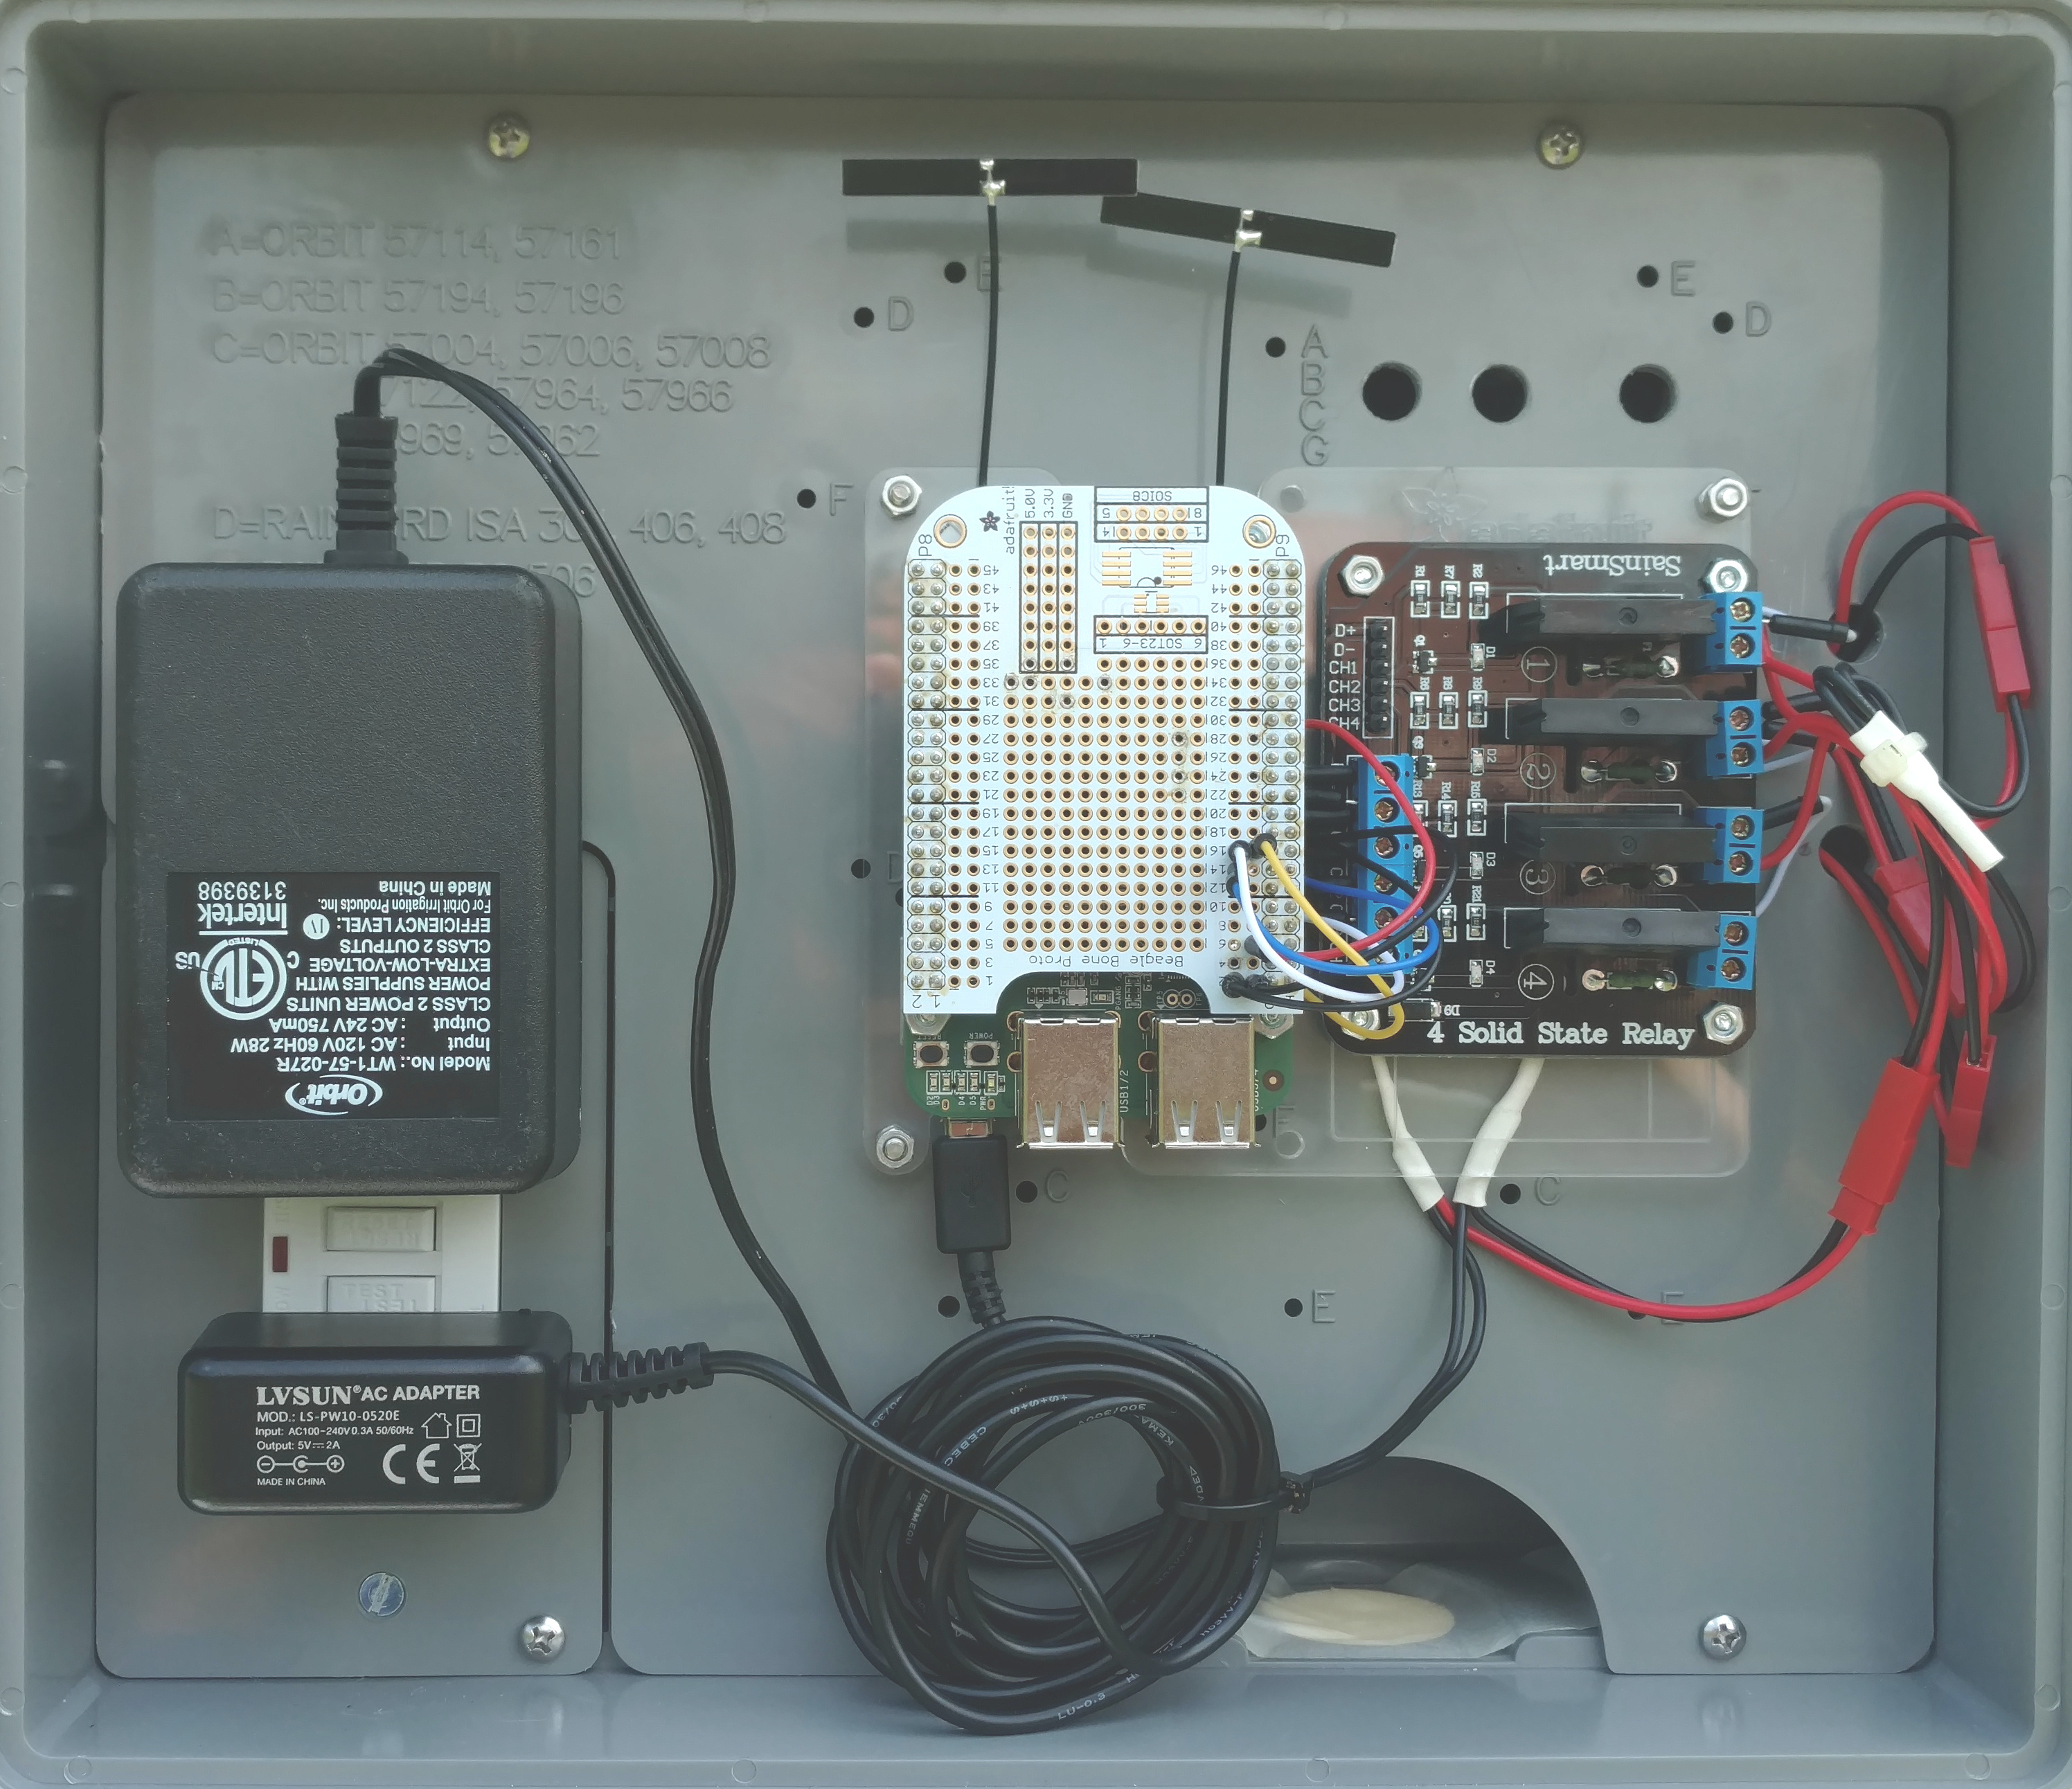
\includegraphics[width=\textwidth]{photos/cover_photo}
\end{figure}

\bigskip
{\centering\bfseries\Large
Gregory Raven
\par}


\bigskip
{\centering\bfseries\LARGE
June 12, 2017
\par}
%\newpage





%\setcounter{page}{1}

%
\frontmatter
Irrigation Controller Using Beaglebone Green Wireless, Node.js, and Ecmascript 6

Copyright 2017 by Gregory Raven

\tableofcontents
\listoffigures

\mainmatter
%    Documentation for PRU ADC Project
%    Copyright (C) 2016  Gregory Raven
%
%    This program is free software: you can redistribute it and/or modify
%    it under the terms of the GNU General Public License as published by
%    the Free Software Foundation, either version 3 of the License, or
%    (at your option) any later version.
%
%    This program is distributed in the hope that it will be useful,
%    but WITHOUT ANY WARRANTY; without even the implied warranty of
%    MERCHANTABILITY or FITNESS FOR A PARTICULAR PURPOSE.  See the
%    GNU General Public License for more details.
%
%    You should have received a copy of the GNU General Public License
%    along with this program.  If not, see <http://www.gnu.org/licenses/>.

\chapter{Introduction}

This is the documentation for an embedded GNU/Linux project utilizing the RemoteProc and RPMsg framework in the Beaglebone Green (BBG) development board.  The project repository is located here:

\url{https://github.com/Greg-R/pru-pid-motor}

The inspiration for this project came from an example project published by Texas Instruments.  The Texas Instruments project is based on "Code Composer Studio", which is an "Integrated Development Environment" (IDE):

\url{http://processors.wiki.ti.com/index.php/PRU_Training:_PRU_PID_Motor_Demo}

There is also a PDF file which describes the project in detail:

\url{http://www.ti.com/lit/ug/tidubj6/tidubj6.pdf}

The TI project requires a relatively complex cross-compiler installation.  This project is designed to be done via SSH terminal connection, and all software compilation was done on the Beaglebone Green target device using the PRU C compiler (clpru).  The VIM text editor was used to edit files, however, any text editor available in the Debian distribution can be used.

The Debian-based GNU/Linux distribution used on the BBG can be downloaded from this page:

\url{http://beagleboard.org/latest-images}

The ``IOT'' (non-GUI) image was chosen, as this provides the shortest path to get the project up and running.

Recent developments in the Texas Instruments PRU support include the RemoteProc and Remote Messaging frameworks, as well as an extensively documented C compiler and much additional supporting documentation.  This project utilizes these frameworks and is entirely dependent upon C code in both the PRU and GNU/Linux user space.  For further information, refer to the detailed examples provided by TI in the ``PRU Support Package'':

\url{https://git.ti.com/pru-software-support-package}

A listing of additional resources is found in the Resources chapter.

The motor recommended by TI was purchased and tested.  However, a better motor with an integrated quadrature encoder was found on eBay and is recommended.  A chapter is included which describes this motor-encoder and how to obtain one.

\section{Project Goals}

This project demonstrates an electronic speed control for a DC motor which is implemented with the PRUs included with the Beaglebone Green.  Beyond its usefulness as a demonstration project, it could be used in a robotics project such as a ``mobile robot''.

The basic principle of the speed controller is "Proportional Integral Derivative" (PID) feedback control, which is a common feedback controller used in digital systems.

Here is an excellent reference article on PID controllers:

\url{http://www.wescottdesign.com/articles/pid/pidWithoutAPhd.pdf}

\section{Limitations}

All of the development was done as root user via ssh on the BeagleBone Green.  This is generally not a good practice, however, considering this as an embedded and experimental project it was not considered to be a serious drawback.

No attempt was made to optimize the response of the PID controller.  The default values for the PID controller create a stable loop with the recommended DC motor-encoder.  Optimization will depend on the particular motor-encoder chosen and this task is left to the interested experimenter.



%    Documentation for PRU ADC Project
%    Copyright (C) 2016  Gregory Raven
%
%    This program is free software: you can redistribute it and/or modify
%    it under the terms of the GNU General Public License as published by
%    the Free Software Foundation, either version 3 of the License, or
%    (at your option) any later version.
%
%    This program is distributed in the hope that it will be useful,
%    but WITHOUT ANY WARRANTY; without even the implied warranty of
%    MERCHANTABILITY or FITNESS FOR A PARTICULAR PURPOSE.  See the
%    GNU General Public License for more details.
%
%    You should have received a copy of the GNU General Public License
%    along with this program.  If not, see <http://www.gnu.org/licenses/>.

\chapter{System Diagrams}

\begin{figure}[H]
	\centering
	\includegraphics[width=0.6\textwidth]{diagrams/system_diagram}
	\centering\bfseries
	\caption{Beagle Bone Green Wireless Irrigation Control System}
\end{figure}

The above diagram shows the main components of the system.  A reference section 
is included which has a complete parts list.


\section{GNU/Linux Operating System on Host ARM Processor}

The command uname -a on the BBG used to develop this project reports this:

\begin{verbatim}
Linux BBG2 4.4.30-ti-r64 #1 SMP Fri Nov 4 21:23:33 UTC 2016 armv7l GNU/Linux
\end{verbatim}

The latest IOT image has a newer kernel.  It is not a major update as of December 18, 2016.







%    Documentation for PRU ADC Project
%    Copyright (C) 2016  Gregory Raven
%
%    This program is free software: you can redistribute it and/or modify
%    it under the terms of the GNU General Public License as published by
%    the Free Software Foundation, either version 3 of the License, or
%    (at your option) any later version.
%
%    This program is distributed in the hope that it will be useful,
%    but WITHOUT ANY WARRANTY; without even the implied warranty of
%    MERCHANTABILITY or FITNESS FOR A PARTICULAR PURPOSE.  See the
%    GNU General Public License for more details.
%
%    You should have received a copy of the GNU General Public License
%    along with this program.  If not, see <http://www.gnu.org/licenses/>.

\chapter{Ecmascript 6}

This page shows which Ecmascript 6 features are implemented in major versions
of Node:

\url{http://node.green/}

Javascript has become a feature rich and large language!
Some of the ES6 constructs used in this project:

\begin{itemize}
\item class
\item Map
\item arrow function
\item Proxy
\item const and let
\end{itemize}

A good reference for ES6 is at the Mozilla Developer Network:

\url{https://developer.mozilla.org/en-US/docs/Web/JavaScript}

A quick summary of the ES6 constructs follows.

\subsection{class}

The new ``class'' keyword does not provide new functionality.  What is does is 
allow a Javascript class object to be written in a more traditional 
object-oriented style.  This does make things easier for a person used to other 
language's syntax for defining classes.

\subsection{Map}

The ``Map'' is a new data structure object which is similar to what is called a 
``hash'', dictionary, or associative array.  Prior to ES6, the Javascript 
object was used functionally as a Map, however, this was kind of a hack.

In this project, the Map object is used in the pumpActuator object.

\subsection{Arrow Function}

``Arrow Functions'' are a simplification of the syntax used when defining a 
function.  However, they are also important in determining the the scope of 
``this'' within the function.  The arrow functions capture the ``this'' of the 
enclosing scope.  This was found to be convenient in the design of the 
pumpActuator class.

\begin{verbatim}
        this.pumpMap = new Map([['pumpmotor', 0],
                              ['zone1', 0],
                              ['zone2', 0]]);
\end{verbatim}

The ``pumpMap'' is a simple data structure to store the state of the pumpmotor 
and the two zone actuators.

\subsection{Proxy}

Of the above ES6 constructs, the only one requiring detailed explanation is the 
``Proxy''.  The construct is used to implement the so-call ``Observer'' pattern.

The instantiation of the ``pumpHashProxy'' is done in the constructor of the 
pumpActuator class:

\begin{verbatim}
        this.pumpHashProxy = new Proxy(this.pumpMap, this.pumpObserver());
\end{verbatim}

The Proxy's constructor takes two arguments, which in this case is this.pumpMap 
and this.pumpObserver().  The second argument requires some explanation.


\begin{verbatim}
    pumpObserver() {
        return {
            set: (target, property, value, receiver) => {
                console.log(`Setting ${property} to ${value}.`);
                this.pumpControl(property, value);
                target[property] = value;
                return true;
            }
        };
    }
\end{verbatim}

The above class method is a little bizarre.  This method merely returns a 
Javascript object.  The object in this case has a single key ``set'' and the 
value is an arrow function with four parameters: target, property, value, and 
receiver.

The Proxy creates a sort of ``watcher'' or ``observer'' of pumpMap.  The proxy 
intercepts changes written to or read from the target object (the first 
parameter of the Proxy constructor).

Using the key ``set'' causes the function (the set key's value) to be executed 
when the value is written to.  Note that the function has access to the 
intercepted property and value, and these are used in call the function 
``this.pumpControl''.  This does the physical setting of the GPIOs.  The data 
structure is also updated (target[property]=value) and ``true'' is returned to 
indicate a successful set.

The proxy does a sort of ``intercept'' of writes to the object and then can 
perform custom actions based on the the function assigned to ``set''.  Similar 
functionality for reads can be done with the ``get'' key.  The object can 
contain both and custom read and write functions can be used.  This is very 
powerful!

Functionally what the Proxy does is intercept the write to the data structure 
which stores the state of the pumpmotor and the zone solenoids.  The intercept 
runs the ``set'' function and changes the physical state of the GPIOs.

The write to the data structure is done by the server in file 
websocketserver.js:

\begin{verbatim}
           Object.assign(pumpObject.pumpHashProxy, controlObject);
\end{verbatim}

The ``controlObject'' in this case is an incoming WebSocket message (using JSON 
notation) from the browser which looks like this example:

\begin{verbatim}
{"pumpmotor":0}
\end{verbatim}

The write to the data structure in the pumpActuator object is done by the 
server in file websocketserver.js:

\begin{verbatim}
           Object.assign(pumpObject.pumpMapProxy, controlObject);
\end{verbatim}

The ``Object.assign'' is a shortcut which simply overwrites the value in 
pumpMapProxy with the value from controlObject.  The Proxy intercepts this 
write, and then executes the custom set function.

The Proxy allows a custom behavior to be executed when a data structure is 
written to or read from.  This is very powerful!  In this particular project 
with only three controls it does not standout, however, this sort of 
``Observer'' pattern is very scalable and could be very advantageous in a much 
larger and more complex system.

\subsection{const and let}

const creates a read-only reference to a block-scoped value.
let is also block-scoped, but it is a variable.

let and const solve the crazy problem of hard to understand scope and 
``hoisting'' of the var type variables of previous versions of Javascript.
 var was not used anywhere in this project.
 
 const and let are a huge improvement to Javascript!




%    Documentation for Irrigation Control Project
%    Copyright (C) 2017  Gregory Raven
%
%    This program is free software: you can redistribute it and/or modify
%    it under the terms of the GNU General Public License as published by
%    the Free Software Foundation, either version 3 of the License, or
%    (at your option) any later version.
%
%    This program is distributed in the hope that it will be useful,
%    but WITHOUT ANY WARRANTY; without even the implied warranty of
%    MERCHANTABILITY or FITNESS FOR A PARTICULAR PURPOSE.  See the
%    GNU General Public License for more details.
%
%    You should have received a copy of the GNU General Public License
%    along with this program.  If not, see <http://www.gnu.org/licenses/>.

\chapter{GPIO Control with sysfs Virtual File System}

This ``sysfs'' virtual file system the core functionality which allows the 
GPIOs to be controlled from user space.

Note that the BBGW must be correctly configured for GPIO output mode on the 
three control pins used to control the irrigation devices.  This document will 
not cover this subject in detail, as this has been well-covered in numerous web 
articles and books.

A highly recommended resource is ``Exploring Beaglebone'' by Derek Molloy.
(add footnote here)

The method of configuring the header pins to GPIO is covered in the chapter 
``Universal IO''.  GPIO configuration must be complete before any of the 
commands shown below will function properly.

``POSIX'' type operating systems, which includes Linux, are ``file based''.  
That means the interface to everything is via writing to or reading from a 
file.  In this case, the GPIO's state is changed by writing a 0 or 1 to the 
appropriate file.  Here is an example:

\begin{verbatim}
echo 1 > /sys/class/gpio/gpio50/value
\end{verbatim}

The above changes the state of header pin P9.14 to ``high'' or an output of 3.3 
volts.  Echoing 0 changes the output to 0.0 volts.  It's that simple!

\subsection{Controlling the GPIOs using Javascript}

The command shown above is typed and executed in a bash shell.  How is this 
done from Javascript?  A module from Node.js is used to accomplish this:

\url{https://nodejs.org/api/child_process.html}

For example, the bash command shown above would be executed as follows in 
Javascript:

\begin{verbatim}
const exec = require('child_process').exec;
exec('echo 1 > /sys/class/gpio/gpio50/value');
\end{verbatim}

This is the simplest possible usage; an optional callback function as a second 
option is possible.  The callback option is used in the in the ``pumpActuator'' 
class, and the callback is used to emit an event from the pumpActuator Object.  
This event is subscribed to by the WebSocket server, and when the event fires 
it sends a message to the web page controller to indicate that the control 
function has changed state.  The web page is updated to indicate the new state.

The class method looks like this:

\begin{verbatim}
    pumpControl(pumpgpio, command) {
        const exec = require('child_process').exec;
        exec(`echo ${command} > ${this.pumpGpioMap.get(pumpgpio)}`, (error, 
        stdout, stderr) => {
            // If error, do not update the status of the controls.
            if (error) {
                console.error(`exec error: ${error}`);
                return;
            } else {
                console.log(`Status message emitted from ledActuator: 
                ${pumpgpio} is set to ${command}.`);
                //  Send a JSON object with the value being an array.
                this.emit('statusmessage', `["${pumpgpio}",${command}]`);
            }
        });
    }
\end{verbatim}








%    Documentation for Irrigation Control Project
%    Copyright (C) 2017  Gregory Raven
%
%    This program is free software: you can redistribute it and/or modify
%    it under the terms of the GNU General Public License as published by
%    the Free Software Foundation, either version 3 of the License, or
%    (at your option) any later version.
%
%    This program is distributed in the hope that it will be useful,
%    but WITHOUT ANY WARRANTY; without even the implied warranty of
%    MERCHANTABILITY or FITNESS FOR A PARTICULAR PURPOSE.  See the
%    GNU General Public License for more details.
%
%    You should have received a copy of the GNU General Public License
%    along with this program.  If not, see <http://www.gnu.org/licenses/>.

\chapter{An HTML5 Controller}

The controller GUI is an HTML5 web page.  The project was developed with the 
Chromium browser in Ubuntu 16.04.

There was no attempt to fix problems with cross-browser compatibility issues.  
Plain HTML5 and CSS was used throughout.  The HTML was manipulated directly via 
the ``Document Object Model'' (DOM) technology in the web browser.  This is a 
bare-bones interface with no fancy features.

\begin{figure}[h]
	\centering
    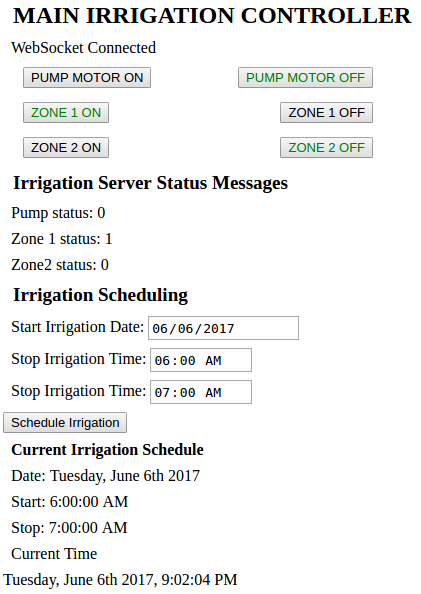
\includegraphics[width=0.5\textwidth]{photos/browser_full.png}
	\centering\bfseries
	\caption{The Irrigation Controller as seen with a Chromium Browser}
\end{figure}

Manual control buttons for the zone solenoids and the pump motor are at the 
top.  The user can enter a schedule date and start and stop times.  Clicking 
the ``Schedule'' button sends the requested irrigation schedule to the server.  
The server responds with a message which updates the displayed schedule.  No 
rigorous checking of inputs is done.

The current date and time are shown in the last line of the controller page.
Originally, the time and date were obtained from the host computer.  This
information is redundant, as the user will have access to the host system time
via some other GUI.  Also, the irrigation timing events will be use the system
time on the BBGW server.  It makes sense to show display the BBGW system time, as
there could be a discrepancy if the BBGW uses a real time clock which has significant
error.

The HTML has been modified to show the BBGW server's system time sent via WebSocket.
The time is updated every minute.  This should be sufficient precision for this
particular application.

%    Documentation for Irrigation Control Project
%    Copyright (C) 2017  Gregory Raven
%
%    This program is free software: you can redistribute it and/or modify
%    it under the terms of the GNU General Public License as published by
%    the Free Software Foundation, either version 3 of the License, or
%    (at your option) any later version.
%
%    This program is distributed in the hope that it will be useful,
%    but WITHOUT ANY WARRANTY; without even the implied warranty of
%    MERCHANTABILITY or FITNESS FOR A PARTICULAR PURPOSE.  See the
%    GNU General Public License for more details.
%
%    You should have received a copy of the GNU General Public License
%    along with this program.  If not, see <http://www.gnu.org/licenses/>.

\chapter{Pump Actuator Class}

The pumpActuator class models the control functions of the irrigation system.  
It extends the Node.js EventEmitter and thus it can emit events.

The class maintains a data structure which stores the current state of the 
system.  This data structure is set up by the class constructor:

\begin{verbatim}
        this.pumpMap = new Map([['pumpmotor', 0],
                              ['zone1', 0],
                              ['zone2', 0]]);
\end{verbatim}

This is an ES6 ``Map'' which is an associative array.  There is a ``key'' for 
the each pump element, and the value of 0 or 1 represents the on or off state.

As explained in the chapter on ES6 a Proxy object is used to implement the 
``Observer'' pattern.

The Proxy can observe changes made to the data structure and execute 
side-effects as required.  In this case, the GPIO state needs to be changed 
each time the pumpMap data structure is updated.  The update can happen via the 
manual controls on the web page, or they can be initiated by the Scheduler 
Object.

The system changes the state of the GPIOs and also updates the status 
indicators on the web page.  This action happens merely by writing to the 
pumpMap data structure.  So it does not matter who does the update; the 
side-effects will always be taken care of automatically.

The class contains another Map which are the paths to the virtual file system 
sys controls for the GPIOs.

The class emits a ``pumpStatusMessage'' whenever a write is done to the pumpMap.
\chapter{Irrigation Scheduler Class}

The Scheduler class is responsible for activating the irrigation system at the 
time specified by the user.  The user enters the start and stop timing using 
the web browser controller.  The watering times are equally split between the 
two zones.

The timing function might seem simple.  However, it proved challenging to 
implement with simple code.

Two excellent Node packages were used:

\url{https://www.npmjs.com/package/node-cron}

and

\url{https://www.npmjs.com/package/moment}

The Node-cron package manager implements a functionality similar to a ``cron 
job'' in a POSIX operating system.  The function provided is a time-delayed 
task set by the user.  In this project, four jobs are required, and thus four 
node-cron tasks are created by a method of the Scheduler class.

The Moment package provides a robust data and time module which is more 
flexible than the native Javascript Date object.  The module's mode of 
operation is a little unusual, however, the documentation is excellent and the 
user should have no problem using the extensive feature set.

\begin{figure}[H]
	\centering
	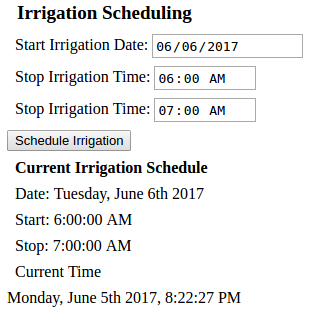
\includegraphics[width=0.6\textwidth]{photos/scheduler.png}
	\centering\bfseries
	\caption{The Web Browser Irrigation Scheduler}
\end{figure}


\chapter{JSON Messaging with WebSocket}

\begin{figure}[h]
	\centering
    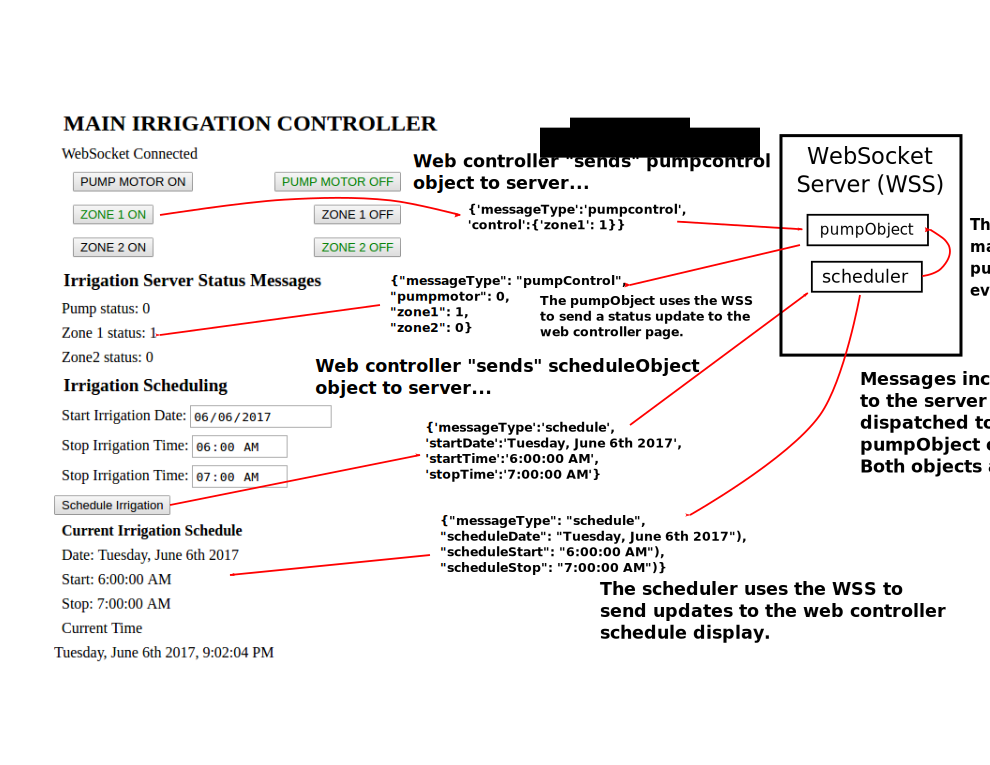
\includegraphics[width=1.0\textwidth]{diagrams/websocket_comms}
	\centering\bfseries
	\caption{JSON Objects are passed between the Web Page Controller and the 
	Server}
\end{figure}

The above diagram shows the flow of data between the web browser controller and 
the BBGW server.

``Javascript Object Notation'' (JSON) is used the format used for the 
messages.  These ``Objects'' are really used as associative arrays would be 
used in other programming languages.  In fact, ES6 includes a formal 
associative array called Map.  However, JSON is a de-facto standard for this 
sort of simple message passing, and the JSON related tools are easy to use.

To send a JSON Object with WebSocket, it is first necessary to ``stringify'' 
the object.  This is done with the JSON.stringify() method.  On the receiving 
end, the JSON.parse() method is used to translate back to a Javascript Object.  
After that, the Object is used with the normal key/value syntax of Javascript.

\section{Example JSON Messages}

Thanks to WebSocket being bidirectional, it is easy to pass messages in both 
directions between the web browser controller and the server.  There are a 
total of four message types; two for browser to server and two for server to 
browser.

\subsection{Browser to Server Hardware Control Message}

This message indicates the device to be controlled and the desired state:

\begin{verbatim}
{'messageType':'pumpControl', 'control':{'zone1':1}}
\end{verbatim}

The key ``messageType'' indicates to the server that this message should be 
routed to the pumpActuator Object.  The ``control'' key's value is another JSON 
object, and this Object has as its key the device to be controlled, and the 
value is the desired state.

A little bit of Javascript trickery is involved to use this piece of incoming 
data:

\begin{verbatim}
Object.assign(pumpObject.pumpMapProxy, dataObject.control);
\end{verbatim}

The pumpActuator object has a data structure containing the current state of 
the zone solenoids and the pump motor.  The data structure is an ES6 ``Map'', 
which is a true associative array.

So what the Object.assign(arg1, arg2) method does is overwrite key:value pair 
located in arg1 with the key:value pair in arg2.

Due to the write being done through a Proxy Object, another function is called 
which physically changes the state of the correct GPIO, and then it sends 
another object back to the web browser to update its status display.

It could be the case that the ES6 Proxy Object will become a preferred method 
for managing state in Javascript based embedded devices.  The interested reader 
is encouraged to check out the documentation at this link:

\url{https://developer.mozilla.org/en-US/docs/Web/JavaScript/Reference/Global_Objects/Proxy}

\subsection{Server to Browser Hardware Status Message}

When the project was first started, the buttons in the web browser to turn the 
hardware components on and off was simple DOM updates of the button colors.

However, this does not indicate the true state of the hardware in the case of a 
communications breakdown between browser and server.

The design was revised to update button indicators only upon receipt of a 
message from the server indicating a successful hardware state change.

The pumpActuator object emits ``pumpStatusMessage'', and then only if a 
WebSocket is open the status message is sent to the browser.  The web browser 
parses the message and uses DOM Javascript manipulation to update the displayed 
hardware status.

\begin{verbatim}
{'messageType':'pumpControl', 'pumpmotor':0, 'zone1':1, 'zone2':0}
\end{verbatim}

\subsection{Browser to Server Scheduling Message}

The system user can input a date, start, and stop times for irrigation to 
happen automatically in the future.  Simple HTML5 form fields are used to 
gather the user's input, and then a ``Schedule Irrigation'' button is clicked.  
If a valid WebSocket is open, a scheduling JSON object is sent to the server.

\begin{verbatim}
{'messageType':'schedule', 'scheduleData':'Tuesday June 6th 2017',
'scheduleStart':'6:00:00 AM', 'scheduleStop':'7:00:00'}
\end{verbatim}

The websocketserver determines the ``messageType'' is schedule, and then 
dispatches the message to the Scheduler Object.  

\subsection{Server to Browser Schedule Display Update Message}

The Scheduler has the necessary logic to drive the hardware per the schedule.

The browser's displayed schedule is updated by the server, not by the browser.  
Thus the server sends the scheduling message back to the browser, but only if 
the message is first processed by the Scheduler object and also a valid 
WebSocket is open.  The message is identical to the browser to server message.

The scheduling display is updated using DOM Javascript methods.
%    Documentation for PRU ADC Project
%    Copyright (C) 2016  Gregory Raven
%
%    This program is free software: you can redistribute it and/or modify
%    it under the terms of the GNU General Public License as published by
%    the Free Software Foundation, either version 3 of the License, or
%    (at your option) any later version.
%
%    This program is distributed in the hope that it will be useful,
%    but WITHOUT ANY WARRANTY; without even the implied warranty of
%    MERCHANTABILITY or FITNESS FOR A PARTICULAR PURPOSE.  See the
%    GNU General Public License for more details.
%
%    You should have received a copy of the GNU General Public License
%    along with this program.  If not, see <http://www.gnu.org/licenses/>.

\chapter{Solid State AC Relays}

\begin{figure}[h]
	\centering
%    \includegraphics[width=0.5\textwidth]{photos/drv8833_breakout.jpg}
	\centering\bfseries
	\caption{DRV8833 Break-out board (2 boards showing with view of top and bottom sides)}
\end{figure}


The recommended motor driver IC is the Texas Instruments DRV8833:

\url{http://www.ti.com/lit/ds/symlink/drv8833.pdf}

This devices works perfectly with this project and is inexpensive.
Several eBay sellers offer a ``break-out board'' with the IC and several external components mounted with break-board friendly header pin holes.  The board shown in the photo above even includes a surface mounted LED power indicator!

The connections to the board are as follows:

\begin{enumerate}
\item ULT PIN:mode set. Low level is sleep mode
\item OUT1,OUT2:1-channel H-bridge controlled by IN1/IN2
\item OUT3,OUT4:2-channel H-bridge controlled by IN3/IN4
\item EEP PIN:Output protection. Default no need to connect.
\item VCC:3-10V
\item GND
\end{enumerate}

From the above list, only 2, 5 and 6 are used in this project.

IN1 is connected to the PWM output of the BBG, which is header P9.42.
The GND pin requires a connection to one of the grounds on the BBG such as P8.1 or P8.2.

VCC should be connected to an 8Volt DC power supply, however, the exact voltage is not critical.  A solid ground connection should be made between the 8Volt supply and the DRV8833 board.

OUT1 and OUT2 should be connected to the motor power terminals.


%    Documentation for Irrigation Control Project
%    Copyright (C) 2017  Gregory Raven
%
%    This program is free software: you can redistribute it and/or modify
%    it under the terms of the GNU General Public License as published by
%    the Free Software Foundation, either version 3 of the License, or
%    (at your option) any later version.
%
%    This program is distributed in the hope that it will be useful,
%    but WITHOUT ANY WARRANTY; without even the implied warranty of
%    MERCHANTABILITY or FITNESS FOR A PARTICULAR PURPOSE.  See the
%    GNU General Public License for more details.
%
%    You should have received a copy of the GNU General Public License
%    along with this program.  If not, see <http://www.gnu.org/licenses/>.

\chapter{Configuration of the Beagle Bone Green Wireless}

The default configuration of the Beagle Bone Green Wireless is as an ``access 
point'' (a wireless router).  This is not a desired configuration for a 
dedicated embedded device as used in this project.

The following process re-configures the BBGW to a non-access point wireless 
mode.

The goal is to have a working wireless substitute for the Ethernet connector 
which does not exist on the BeagleBone Green Wireless.
This is as a typical "headless" embedded project with the primary access using 
a terminal and ssh.

\section{Get Latest IOT Image}

Download and expand the IOT bone image per this link and flash to micro-sd.  I 
used this one:

\url{https://debian.beagleboard.org/images/bone-debian-8.7-iot-armhf-2017-03-19-4gb.img.xz}

Write the image to the micro-sd (I put the micro-sd in a USB adapter plugged 
into my Ubuntu workstation):

\begin{verbatim}
xzcat bone-debian-8.7-iot-armhf-2017-03-19-4gb.img.xz | sudo dd of=/def/sdb
\end{verbatim}

Eject the micro-sd from workstation and insert in the BBGW micro-sd slot.
Connect a USB 3.3V serial device to the "debug serial header".  The USB network 
connection could be substituted, however, my experience
with this is that using the serial device is solid and will work consistently.
Also, the BBGW doesn't have a dedicated power connector.  It uses the 
micro-USB.
It is my preference to use a dedicated USB power supply and ignore 
USB as a network connection.

Power-up the BBGW and wait for the boot process to complete.
Open a (bash) terminal and use the screen utility to connect via the serial USB 
device.

\begin{verbatim}
screen /dev/ttyUSB0 115200
\end{verbatim}

I had to hit enter after the above command to get to the login prompt.
The login user is debian and the password is temppwd.

You may have to install screen:

\begin{verbatim}
sudo apt-get install screen
\end{verbatim}

After logging in the first time, a good thing to do first is to run this shell 
script:

\begin{verbatim}
cd /opt/scripts/tools
sudo ./grow_partition.sh
\end{verbatim}

\section{Enable the BBGW Universal Cape}

The file /boot/uEnv.txt must be edited to enable the BBGW universal cape.  This 
will set up the GPIOs at boot time.

Using root access, open the file /boot/uEnv.txt.
Find this section of the file:

\begin{verbatim}
##Example v4.1.x
#cape_disable=bone_capemgr.disable_partno=
#cape_enable=bone_capemgr.enable_partno=
\end{verbatim}

Edit the cape\_enable line to look like this:

\begin{verbatim}
##Example v4.1.x
#cape_disable=bone_capemgr.disable_partno=
cape_enable=bone_capemgr.enable_partno=univ-bbgw
\end{verbatim}

The change will take effect upon next boot.

\section{Wireless Network Configuration}

Enter this command:

\begin{verbatim}
if addr
\end{verbatim}

You should see 4 different network resources (not showing the full output here):

\begin{verbatim}
SoftAp0
lo
usb0
wlan0
\end{verbatim}

The network resource SoftAp0 represents an "access point".
The BBGW is configured as a wireless router!
That is not the desired configuration, and fortunately this is easily removed.
Edit the file:

\begin{verbatim}
/etc/default/bb-wl18xx
\end{verbatim}

Change the line:

\begin{verbatim}
TETHER_ENABLED=yes
\end{verbatim}

to

\begin{verbatim}
TETHER_ENABLED=no
\end{verbatim}

Save and exit, and reboot, and login.

ifconfig should now show only 3:  lo, usb0, and wlan0.

Now to configure WIFI!  It is assumed you have a home wireless router and you 
know the SSID and passphrase.
The router should be configured for DHCP (automatic assignment of IP addresses).
From a terminal:

\begin{verbatim}
sudo connmanctl
connmanctl> scan wifi
Scan completed for wifi
connmanctl> services
    (your router broadcast)         (router info)
connmanctl> agent on
Agent registered
connmanctl> connect (copy router info here)
Agent RequestInput (router info)
  Passphrase = [ Type=psk, Requirement=mandatory, Alternates=[ WPS ] ]
  WPS = [ Type=wpspin, Requirement=alternate ]
Passphrase? (your passphrase)
Connected (router info)
connmanctl> quit
\end{verbatim}

The above configuration is permanent and will survive reboot.
An outstanding page with good info on connman:

\url{https://wiki.archlinux.org/index.php/Connman}

Next, login to your router and use this to determine if 
your BBGW is successfully connected.
Remember the router may have security settings which may block it from 
connecting.  Change this as required.
Also, rather than attempting to force a fixed IP address on the BBGW, I used 
the "address reservation" feature
so that the IP address assigned by the router will be the same each time it 
connects.  This is done using the MAC address of the BBGW.

After the above configuration is done, shutdown and remove the USB serial 
device.
Power up the BBGW and wait for it to boot, and then using a terminal and ssh 
you should be able to connect to the BBGW as if an ethernet cable was connected:

ssh debian@(the assigned IP address)

After logging in you should have internet connectivity, so don't forget to:

\begin{verbatim}
sudo apt-get update
\end{verbatim}

\section{Copy Public SSH Key to BBGW}

Another good thing to do is to copy your public ssh key to the BBGW:

\begin{verbatim}
ssh-copy-id -i id\_rsa.pub debian@192.168.1.3
\end{verbatim}

where you need to substitute the IP address assigned to the BBGW by the 
router.  This will allow you to bypass the usual login authentication routine.

\section{USB Serial Device}

Here is an example USB serial device.  This should be on your tool kit list:

\url{https://www.amazon.com/gp/product/B01AFQ00G2/ref=oh_aui_search_detailpage?ie=UTF8&psc=1}

\section{Change of Wireless Router}

If the home wireless router is re-configured or replaced, this could require 
the use of the serial USB device again.  That's a problem assuming the device 
is remote mounted.

One possibility is to configure the new WIFI router for deployment in the home 
network and place it in range of the BBGW.  Using the above procedure for 
wireless network configuration, the router information for the new router is 
copied into the configuration while still connected with the old router.

As soon as the correct passphrase is entered the connection to the former 
router will drop.  The new router can now be deployed and the BBGW will connect 
to it.

\section{Flash the eMMC After Completing Development}

Running the GNU/Linux OS and applications from the SD card is OK for 
development purposes.  However, using an SD card is not a reliable long-term 
solution.

It is better to flash the contents of the SD card to the on-board eMMC flash 
drive.  This device is specifically designed for use with an operating system 
and will adapt and survive as the memory cells wear out.

A simple change to a file on the microSD card will cause the flash process to 
commence upon the next boot-up.  From the Beagleboard web site:

\begin{quotation}
To turn these images into eMMC flasher images, edit the /boot/uEnv.txt file on 
the Linux partition on the microSD card and remove the '\#' on the line with 
'cmdline=init=/opt/scripts/tools/eMMC/init-eMMC-flasher-v3.sh'. Enabling this 
will cause booting the microSD card to flash the eMMC. Images are no longer 
provided here for this to avoid people accidentally overwriting their eMMC 
flash.
\end{quotation}

The above process will take a few minutes to complete.  You may observe a 
special pattern (back and forth ``cylon'') of the LEDs flashing during the 
process.

When the process is complete, the board will shut itself down.

\textbf{Very important!  Remove the microSD card from its slot or the process 
will repeat upon next boot!}

Label and store the microSD card in a safe place.








\chapter{I2C Real Time Clock}

The Beaglebone series of development boards does not include a ``real time clock'' with a battery back-up.  The included real time clock only functions while power is applied to the board.

When a Linux based device has connectivity to the internet, it can access the current time via ``Network Time Protocol'' (NTP).  These are servers which are maintained with very precise timing.

The Debian distribution used with the BBGW includes NTP already up and running.  The Beaglebone's own real time clock is synchronized using NTP at boot.  However, if boot occurs with no access to internet, the real time clock will have a large error.

A hardware ``real time clock'' can be added to provide accurate timing to the board even if the internet connection is down.  A lithium battery powers the real time clock even when power is removed from the BBGW.

Please note that this subject of time, date, and clocks can get quite complex!  Linux has several mechanisms and services for tracking date and time and keeping everything synchronized, and this can get rather confusing.

The following real time clock module is suggested:

\url{https://www.seeedstudio.com/Grove-High-Precision-RTC-p-2741.html}

The clock has a ``Grove'' connector and cable and easily plugs into the BBGW.

You will need to also purchase a CR1225 3.3volt coin cell battery.

Install the battery in the RTC, and plug it into the I2C Grove connector on the BBGW.  This is the Grove connector closest to P9.  The other Grove connector is for UART.

Power up the BBGW and log in.  Try this command at the command line:

\begin{verbatim}
i2cdetect -y -r 2
\end{verbatim}

You should see this:

\begin{verbatim}
     0  1  2  3  4  5  6  7  8  9  a  b  c  d  e  f
     00:          -- -- -- -- -- -- -- -- -- -- -- -- -- 
     10: -- -- -- -- -- -- -- -- -- -- -- -- -- -- -- -- 
     20: -- -- -- -- -- -- -- -- -- -- -- -- -- -- -- -- 
     30: -- -- -- -- -- -- -- -- -- -- -- -- -- -- -- -- 
     40: -- -- -- -- -- -- -- -- -- -- -- -- -- -- -- -- 
     50: -- 51 -- -- UU UU UU UU -- -- -- -- -- -- -- -- 
     60: -- -- -- -- -- -- -- -- -- -- -- -- -- -- -- -- 
     70: -- -- -- -- -- -- -- --
\end{verbatim}

The above output from i2cdetect indicates the RTC is successfully installed and communicating via I2C bus.

Now permanently ``install'' the I2C device with this command:

\begin{verbatim}
sudo sh -c 'echo pcf85063 0x51 > /sys/class/i2c-adapter/i2c-2/new_device'
\end{verbatim}

Now see if the real time clock installed successfully:

\begin{verbatim}
cat /sys/class/rtc/rtc1/name
\end{verbatim}

This should return:

\begin{verbatim}
rtc-pcf85063
\end{verbatim}

Now read back the time from the new RTC:

\begin{verbatim}
sudo hwclock -r -f /dev/rtc1
\end{verbatim}

You will probably get something like this:

\begin{verbatim}
Sat 01 Jan 2000 12:24:47 AM EST  -0.582551 seconds
\end{verbatim}

Now the RTC must be ``set''.  The following assumes that the BBGW is connected to the internet, and it is using the ``Network Time Protocol'' service which was implemented by default in the image used for this project.
To check this, use this command:

\begin{verbatim}
timedatectl
\end{verbatim}

This will return something like this:

\begin{verbatim}
      Local time: Sat 2017-07-15 19:24:20 EDT
      Universal time: Sat 2017-07-15 23:24:20 UTC
      RTC time: Sat 2017-07-15 23:24:21
      Time zone: America/New_York (EDT, -0400)
      Network time on: yes
      NTP synchronized: yes
      RTC in local TZ: no
\end{verbatim}

This indicates that the automatic synchronization to NTP is enabled.

Next, the RTC must be set to the I2C device.  This is accomplished by the addition of a new file to the udev rules:

\begin{verbatim}
sudo sh -c 'echo "SUBSYSTEM=="rtc", KERNEL=="rtc1", SYMLINK+="rtc", OPTIONS+="link_priority=10", TAG+="systemd"" > /etc/udev/rules.d/51-i2c-rtc.rules'
\end{verbatim}

This command will indicate if the time setting was successful:

\begin{verbatim}
timedatectl
\end{verbatim}

If the time setting was successful, use this command to write to the RTC:

\begin{verbatim}
hwclock -w -f /dev/rtc1
\end{verbatim}

Now check the real time clock:

\begin{verbatim}
hwclock -r -f /dev/rtc1
\end{verbatim}

The above process will not be preserved upon next boot-up.  It is necessary to create a ``service'' and start it each time the board is booted.  Fortunately this is simple to accomplish.

A bash script which duplicates the set-up described above is included in the software directory:

\begin{verbatim}
#!/bin/bash

sleep 15
echo ds1307 0x68 > /sys/class/i2c-adapter/i2c-2/new_device
hwclock -s -f /dev/rtc1
hwclock -w
\end{verbatim}

The above process was based on this information at Adafruit:

\url{https://learn.adafruit.com/adding-a-real-time-clock-to-beaglebone-black/set-rtc-time}



%    Documentation for PRU ADC Project
%    Copyright (C) 2016  Gregory Raven
%
%    This program is free software: you can redistribute it and/or modify
%    it under the terms of the GNU General Public License as published by
%    the Free Software Foundation, either version 3 of the License, or
%    (at your option) any later version.
%
%    This program is distributed in the hope that it will be useful,
%    but WITHOUT ANY WARRANTY; without even the implied warranty of
%    MERCHANTABILITY or FITNESS FOR A PARTICULAR PURPOSE.  See the
%    GNU General Public License for more details.
%
%    You should have received a copy of the GNU General Public License
%    along with this program.  If not, see <http://www.gnu.org/licenses/>.

\chapter{Device Tree Requirements}

This project requires only three GPIOs.  Rather than editing device tree files, 
and having to deal with potential bugs caused by this, the great config-pin 
utility was used.  This utility is provided by the Universal IO project.

The Universal IO project is located at this Github repository:

\url{https://github.com/cdsteinkuehler/beaglebone-universal-io}

Universal IO is included with the most recent Debian-based IOT images.





%    Documentation for Irrigation Control Project
%    Copyright (C) 2017  Gregory Raven
%
%    This program is free software: you can redistribute it and/or modify
%    it under the terms of the GNU General Public License as published by
%    the Free Software Foundation, either version 3 of the License, or
%    (at your option) any later version.
%
%    This program is distributed in the hope that it will be useful,
%    but WITHOUT ANY WARRANTY; without even the implied warranty of
%    MERCHANTABILITY or FITNESS FOR A PARTICULAR PURPOSE.  See the
%    GNU General Public License for more details.
%
%    You should have received a copy of the GNU General Public License
%    along with this program.  If not, see <http://www.gnu.org/licenses/>.

\chapter{Setting the BBGW to Local Time}

The default time setting of the BBGW was found to be UTC.  It was desired to 
have this set to local time.

Fortunately, there is a web page by Derek Molloy which covers this subject in 
detail:

\url{http://derekmolloy.ie/automatically-setting-the-beaglebone-black-time-using-ntp/}

The change to local time is done by removing an existing file, and then adding 
a symbolic link:

\begin{verbatim}
cd /etc
rm localtime
ln -s /usr/share/zoneinfo/America/New_York /etc/localtime
\end{verbatim}

In the above example, the time zone is set to North America Eastern (New 
York).  A complete listing of the possibilities is found in/usr/share/zoneinfo.
Simply find the appropriate path for your time zone and create the link.

The time zone setting will take effect upon the next boot.

Note that the BBGW does not have a local clock source.  It obtains timing data 
via the ``Network Time Protocol''.  It must have internet access for this to 
function.

%    Documentation for PRU ADC Project
%    Copyright (C) 2016  Gregory Raven
%
%    This program is free software: you can redistribute it and/or modify
%    it under the terms of the GNU General Public License as published by
%    the Free Software Foundation, either version 3 of the License, or
%    (at your option) any later version.
%
%    This program is distributed in the hope that it will be useful,
%    but WITHOUT ANY WARRANTY; without even the implied warranty of
%    MERCHANTABILITY or FITNESS FOR A PARTICULAR PURPOSE.  See the
%    GNU General Public License for more details.
%
%    You should have received a copy of the GNU General Public License
%    along with this program.  If not, see <http://www.gnu.org/licenses/>.

\chapter{Running the Project}

Running the project at the command line, starting from the top of the git 
repository:

git clone https://github.com/Greg-R/irrigate-control.git
cd irrigate-control
cd software/node
npm install --save

The above should install the Node packages into a directory ``node\_modules''.






 

%    Documentation for Irrigation Control Project
%    Copyright (C) 2017  Gregory Raven
%
%    This program is free software: you can redistribute it and/or modify
%    it under the terms of the GNU General Public License as published by
%    the Free Software Foundation, either version 3 of the License, or
%    (at your option) any later version.
%
%    This program is distributed in the hope that it will be useful,
%    but WITHOUT ANY WARRANTY; without even the implied warranty of
%    MERCHANTABILITY or FITNESS FOR A PARTICULAR PURPOSE.  See the
%    GNU General Public License for more details.
%
%    You should have received a copy of the GNU General Public License
%    along with this program.  If not, see <http://www.gnu.org/licenses/>.

\chapter{Setting up a systemd Irrigation Service}

systemd is responsible for booting up the user space in Debian (and other) 
GNU/Linux distributions including the BBGW.

This system can be used to start the Node.js server as an ``irrigation'' 
service.

This is easy to accomplish and can be done by creating a single text file:

\begin{verbatim}
/etc/systemd/system/irrigation.service
\end{verbatim}

The file is located in the git repository systemd folder.
Here is the contents of the file irrigation.service:

\begin{verbatim}
[Unit]
Description=Irrigation Control Server

[Service]
ExecStart=/usr/bin/node /home/debian/irrigate-control/software/node/server.js

[Install]
WantedBy=graphical.target
\end{verbatim}

The [Unit] section provides a short description of the service which is printed 
out when the service is interrogated.

The [Service] section is the complete path to the node command followed by the 
path to the server.js file.  This is the ``service'' which will be 
``daemonized'' at boot.

The [Install] section indicates the default state in which the service should 
be started.  The default state can be found by using this command:

\begin{verbatim}
systemctl get-default
\end{verbatim}

In the case of the IOT distribution used by this project, the response is:

\begin{verbatim}
graphical.target
\end{verbatim}

Once the service unit file is in place, enable the service like this:

\begin{verbatim}
systemctl enable irrigation
\end{verbatim}

The irrigation service will now start at boot time!  Set a bookmark in your 
browser, and simply click to go straight to the irrigation control page.

To permanently disable the service:

\begin{verbatim}
systemctl disable irrigation
\end{verbatim}

When debugging, it may be necessary to temporarily stop the service.  Use this 
command:

\begin{verbatim}
systemctl stop irrigation
\end{verbatim}

To start the service again:

\begin{verbatim}
systemctl start irrigation
\end{verbatim}




%    Documentation for PRU ADC Project
%    Copyright (C) 2016  Gregory Raven
%
%    This program is free software: you can redistribute it and/or modify
%    it under the terms of the GNU General Public License as published by
%    the Free Software Foundation, either version 3 of the License, or
%    (at your option) any later version.
%
%    This program is distributed in the hope that it will be useful,
%    but WITHOUT ANY WARRANTY; without even the implied warranty of
%    MERCHANTABILITY or FITNESS FOR A PARTICULAR PURPOSE.  See the
%    GNU General Public License for more details.
%
%    You should have received a copy of the GNU General Public License
%    along with this program.  If not, see <http://www.gnu.org/licenses/>.

\chapter{Resources}

\section{Github repository for this project}

\url{https://github.com/Greg-R/}



\section{Beagle Bone Green Wireless}

\url{https://www.seeedstudio.com/SeeedStudio-BeagleBone-Green-Wireless-p-2650.html}




\backmatter
% bibliography, glossary and index would go here.

\end{document}
